\documentclass[handout]{beamer}

\usetheme[progressbar=frametitle]{metropolis}
\metroset{block=fill}

\subtitle{NTIN071 Automata and Grammars}
\author{Jakub Bulín (KTIML MFF UK)}

\date{Spring 2025\\ 
    \vspace{1in} 
    \begin{flushleft}
        \it \footnotesize * Adapted from the Czech-lecture slides by Marta Vomlelová with gratitude. The translation, some modifications, and all errors are mine.
    \end{flushleft}
}

%% packages

\usepackage{amsmath}
\usepackage{amssymb}
\usepackage{amsthm}
\usepackage{cancel}
\usepackage{color}
\usepackage{colortbl}
\usepackage{forest}
\usepackage[utf8x]{inputenc}
\usepackage{multicol}
\usepackage{multirow}

%% colors
\definecolor{Gray}{gray}{0.9}

%% TikZ
\usepackage{tikz}
    \usetikzlibrary{
        automata,
        arrows,
        backgrounds,
        decorations.pathmorphing,
        fit,
        positioning,
        shapes,
        shapes.geometric,
        tikzmark
    } 
    \tikzset{>=stealth',shorten >=1pt,auto,node distance=2cm}
    \tikzset{initial text={}}
    \tikzset{elliptic state/.style={draw,ellipse}}

%% amsthm
\theoremstyle{plain}
    \newtheorem*{algorithm}{Algorithm}    
    \newtheorem*{observation}{Observation}
    \newtheorem*{proposition}{Proposition}

\theoremstyle{remark}
    \newtheorem*{exercise}{Exercise}
    \newtheorem*{remark}{Remark}

%% macros
\DeclareMathOperator{\RegE}{RegE}
\DeclareMathOperator{\RL}{RL}

% Just for Lecture 2
\newcommand{\x}{$\times$}
\newcommand{\nx}{\ }



\title{Lecture 2 -- Myhill--Nerode theorem, Equivalent and Minimal Representations}


\begin{document}


\frame{\titlepage}


\begin{frame}{Recap of Lecture 1}

    \begin{itemize}
        \item  \alert{Deterministic Finite Automaton (DFA)}: $A=(Q,\Sigma,\delta,q_0,F)$
        \item Extended transition function $\delta^*$
        \item The language \alert{recognized} by the DFA $A$ is the language 
        $$
        L(A)=\{w\in \Sigma^* \mid \delta^*(q_0,w)\in F\}
        $$    
        \item Languages recognized by some DFA are called \alert{regular}
        \item Finite automata encode only finite information, but can recognize infinite languages
        \item Product automaton, intersection of reg. languages is regular      
        \item \alert{Pumping lemma for regular languages} (prove nonregularity)
        \item PL not a characterization, some nonregular can be pumped
        \item A language is infinite iff it contains a word of length $n\leq |w|\leq 2n$ where $n=\#\text{states}$ of a recognizing automaton
    \end{itemize}

\end{frame}


\section{1.4 Myhill--Nerode Theorem}


\begin{frame}{Characterize regular languages}

    How to recognize if a given language is regular? So far, we can construct a DFA recognizing the language, or use the Pumping lemma for contradiction. 
    
    We would like to have a \alert{characterization} (which the Pumping Lemma is not!).

    Luckily, as we'll see, every regular language comes with an implicit automaton `hiding' in the set of all words over its alphabet.

\end{frame}


\begin{frame}{Congruences on words}

    Let $\Sigma$ be a finite alphabet and $\sim$ an equivalence relation on $\Sigma^*$ (reflexive, symmetric, transitive). Then:
    
    \begin{itemize}
        \item $\sim$ is a \alert{right congruence} iff $(\forall u,v,w\in \Sigma^*) u\sim v \Rightarrow uw\sim vw $.
        \item $\sim$ has \alert{finite index} iff the partition $\Sigma^*/\sim$ has a finite number of classes.
        \item the class containing a word $u$ is denoted \alert{$[u]_{\sim}$} or simply $[u]$
    \end{itemize}

\end{frame}


\begin{frame}{The theorem}

    \begin{theorem}[Mihyl--Nerode theorem]
        Let $\Sigma$ be a finite alphabet and $L \subset \Sigma^*$ a language over $\Sigma$. The following statements are
        equivalent:
            \begin{enumerate}[(i)]
                \item $L$ is regular,
                \item there exists a right congruence $\sim$ on $\Sigma^*$ with finite index such that $L$ is a union of some classes of the partition $\Sigma^*/\sim$.
            \end{enumerate}
    \end{theorem}

    \textbf{Proof idea:} Group together words that end in the same state when we start reading from $q_0$.

\end{frame}


\begin{frame}{The proof}

    \alert{(i){\Large$\Rightarrow$}(ii)} from an automaton to a right congruence of finite index
    \vspace{-6pt}
    \begin{itemize}
        \item we define \alert{$u\sim v \equiv \delta^*(q_0,u)=\delta^*(q_0,v)$}
        \item it is indeed a right congruence (from the definition of  $\delta^*$)
        \item it has a finite index ($Q$ is finite)
        \item $L=\{w \mid \delta^*(q_0,w)\in F\}=\bigcup_{q\in F}\{w\mid \delta^*(q_0,w)=q\}$ {$ =\bigcup_{q\in F} [w \mid \delta^*(q_0,w)=q]_\sim$} .
    \end{itemize}

    \vspace{-6pt}
    \alert{(ii){\Large$\Rightarrow$}(i)} from a right congruence of finite index to an automaton
    \vspace{-6pt}
    \begin{itemize}
        \item the alphabet is $\Sigma$, states \alert{$Q$ are the congruence classes $\Sigma^*/\sim$}
        \item the initial state $q_0=[\lambda]$, final states $F=\{c_1, \ldots, c_n\}$ where $L=\bigcup_{i=1,\ldots,n}c_i$
        \item trans. function \alert{$\delta([u],x)=[ux]$} {(well-defined right congruence)}
        \item to show that $L(A)=L$, using $\delta^*([\lambda],w)=[w]$: 
        
        \alert{$w\in L$} $\Leftrightarrow$ $w\in \bigcup_{i=1,\ldots,n}c_i$ $\Leftrightarrow$ $w\in c_1 \vee \ldots w\in c_n$ $\Leftrightarrow$ $[w]=c_1 \vee \ldots [w]=c_n$ $\Leftrightarrow$ $[w]\in F$ $\Leftrightarrow$ \alert{$w\in L(A)$}
        \hfill\qedsymbol
    \end{itemize}

\end{frame}


\begin{frame}{Application: proof of regularity}

    \begin{example}
        Construct an automaton that recognizes the language $L=\{w\in\{a,b\}^* \mid  |w|_{a}=3k+2\text{ for some }k\geq 0\}$.
    \end{example}    
    \vspace{-12pt}
    $$
    u\sim v \text{ iff } |u|_a \equiv |v|_a \pmod{3}
    $$
    \vspace{-16pt}
    \begin{itemize}
        \item equivalence classes are 0,1,2
        \item $L$ corresponds to the class 2
        \item a -- transitions to the next class
        \item b -- stay in the same class.
    \end{itemize}
    
    \begin{center}
        \scalebox{0.9}{
            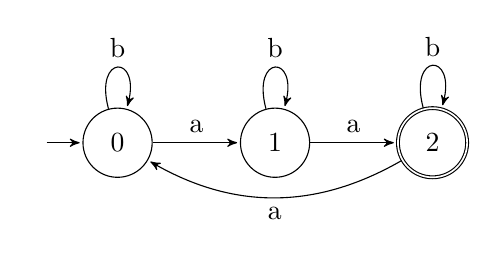
\begin{tikzpicture}[>=stealth',shorten >=1pt,auto,node distance=2cm]
                \node[initial,state] (a)      {0};
                \node[state] (b)  [right of=a]    {1};
                \node[state,accepting] [right of=b](c)      {2};
                \path[->]
                    (a)  edge  node {a} (b)
                    (b)  edge  node {a} (c)
                    (c)  edge [bend left]  node {a} (a)
                    (a)  edge [loop above] node {b} (a)
                    (b)  edge [loop above] node {b} (b)
                    (c)  edge [loop above] node {b} (c)
                ;
            \end{tikzpicture}
        }
    \end{center}        

\end{frame}


\begin{frame}{Application: proof of nonregularity}

    \begin{example}
        Show that $L=\{u\in\{a,b,c\}^*\mid u=a^+b^ic^i \text{ or } u=b^ic^j\}$ is not regular. (Note that the first letter can be pumped.)
    \end{example}

    Suppose for contradiction that $L$ is regular. Let $\sim_{L}$ be a right congruence of finite index where $L$ is a union of some $\sim_{L}$-classes.
        
    Consider the set of words $S=\{a,ab,abb,\ldots\}=\{ab^n\mid n\in\mathbb N\}$.
    
    For any two $i\neq j$ there is a string ($c^i$) distinguishing the words (in/out of the language): $ab^ic^i\in L$ but $ab^jc^i\notin L$
    
    No two elements of $S$ can be in the same class of  $\sim_{L}$ ($L$ would split the class). Since $S$ is infinite, this contradicts finite index of $\sim_{L}$.\hfill\qedsymbol

\end{frame}


\section{1.5 Equivalent and Minimal Representations}


\begin{frame}{Equivalent automata}

    \begin{definition}
        Finite automata $A,B$ are \alert{equivalent} iff they recognize the same language, that is $L(A)=L(B)$.
    \end{definition}
       
    \begin{example} 
        $L=\{w\in \{1\}^*\mid |w|=3k\text{ for some }k\geq 0\}$
    \end{example}
       
    \begin{center}
        \scalebox{0.9}{
            \begin{tikzpicture}[>=stealth',shorten >=1pt,auto,node distance=2cm]
                \tikzset{every state/.style={minimum size=0.2cm}}
                \node[initial,state,accepting] (a) {};
                \node[state] (b)  [above right of=a] {};
                \node[state] [below right of=b](c) {};
                \node[initial,state,accepting] [right=4cm of a] (a1) {};
                \node[state] (b1)  [above right of=a1] {};
                \node[state] [right of=b1](c1) {};
                \node[state,accepting] [right=4cm of a1] (a2) {};
                    \node[state] (b2)  [below right of=a1] {};
                        \node[state] [right of=b2](c2) {};
                \path[->]
                    (a)  edge  node {1} (b)
                    (b)  edge  node {1} (c)
                    (c)  edge   node {1} (a)
                    (a1)  edge  node {1} (b1)
                    (b1)  edge  node {1} (c1)
                    (c1)  edge   node {1} (a2)
                    (a2)  edge  node {1} (c2)
                    (b2)  edge  node {1} (a1)
                    (c2)  edge  node {1} (b2)
                ;
            \end{tikzpicture}
        }
    \end{center}           

\end{frame}


\begin{frame}{Automata homomorphism}

    \begin{definition}
        Let $A_1,A_2$ be DFAs. A surjective mapping $h: Q_1\rightarrow Q_2$ is an \alert{(automata) homomorphism}, if it satisfies:
        \begin{itemize}
            \item $h(\delta_1(q,x))=\delta_2(h(q),x)$
            \item $h(q_{0_1})=q_{0_2}$            
            \item $q\in F_1 \Leftrightarrow h(q)\in F_2$
        \end{itemize}
        A bijective homomorphism is called an \alert{isomorphism}.
    \end{definition}

    (Isomorphic automata only differ by the `names' of the states.)

    \medskip

    \begin{theorem}[Automata Equivalence Theorem]
        Let $A_1,A_2$ be DFAs. If there exists a homomorphism from $A_1$ to $A_2$, then $A_1$ and $A_2$ are equivalent.
    \end{theorem}

\end{frame}


\begin{frame}{The proof}

    For any $w\in \Sigma^*$, $q\in Q_1$, we can prove by finite induction that 
	$$
    h(\delta_1^*(q,w))=\delta_2^*(h(q),w)
    $$
    Then the following holds:

    \begin{columns}

        \column{0.65\textwidth}

        \begin{eqnarray*}
            w\in L(A_1)&\Leftrightarrow&\delta_1^*(q_{0_1},w)\in F_1\\
            &\Leftrightarrow&h(\delta_1^*(q_{0_1},w))\in F_2\\
            &\Leftrightarrow&\delta_2^*(h(q_{0_1}),w)\in F_2\\
            &\Leftrightarrow&\delta_2^*(q_{0_2},w)\in F_2\\
            &\Leftrightarrow&w\in L(A_2)
        \end{eqnarray*}

        \column{0.35\textwidth}

        \begin{center}
            \scalebox{0.9}{
                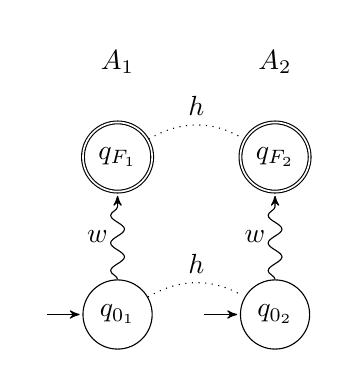
\begin{tikzpicture}
                    \node[initial,state] (a)      {$q_{0_1}$};
                    \node[state,accepting] (g)  [above of=a]     {$q_{F_1}$};
                    \node[initial,state] (a2)   [right of=a]   {$q_{0_2}$};
                    \node[state,accepting] (g2)  [above of=a2]     {$q_{F_2}$};
                    \node[state,draw=none] (d1)  [above=0.3cm of g]    {$A_1$};
                    \node[state,draw=none] (d2)  [above=0.3cm of g2]    {$A_2$};
                    \path[->]
                        (a)  edge[decorate,decoration=snake]  node {$w$} (g)
                        (a2)  edge[decorate,decoration=snake]  node {$w$} (g2)
                        (a)  edge[-,dotted,bend left]  node {$h$} (a2)
                        (g)  edge[-,dotted,bend left]  node {$h$} (g2)
                    ;
                    %\draw [->,decorate,decoration=snake] (0,0) -- (2,0);
                \end{tikzpicture}
            }
        \end{center}        
        \hfill\qedsymbol        
    \end{columns}

\end{frame}


\begin{frame}{Reducing automata}

    The smallest DFA recognizing a given language?

    Start with any DFA.

    Two steps:

    \begin{itemize}
        \item remove \alert{unreachable} states
        \item merge \alert{equivalent (indistinguishable)} states
    \end{itemize}

    The reduced DFA is unique (up to automata isomorphism).

\end{frame}


\begin{frame}{(Un)reachable states}

    \begin{definition}[Reachable states]
        Let's have a DFA $A=(Q,\Sigma,\delta,q_0,F)$ and $q\in Q$. The state $q$ is \alert{reachable} iff there exists $w\in \Sigma^*$ such that $\delta^*(q_0,w)=q$. 
        \end{definition}
        
        \begin{algorithm}[Reachable States -- BFS on the state diagram]        
            \begin{itemize}
                \item set $M_0=\{q_0\}$
                \item repeat $M_{i+1}=M_i \cup \{q\in Q\mid (\exists p\in M_i, \exists x\in \Sigma)\ \delta(p,x)=q\}$
                \item until $M_{i+1}=M_i$
                \item return $M_i$
            \end{itemize}
        \end{algorithm}
        \begin{proof}[Proof of correctness and completeness]
           \alert{Corectness:} $M_0\subseteq M_1\subseteq \ldots\subseteq Q$ and consist of reachable states.
            \alert{Completeness:} Let $q$ be reachable. Let $w=x_1\ldots x_n$ be shortest such that $\delta^*(q_0,x_1\ldots x_n)=q$. As $\delta^*(q_0,x_1\ldots x_i)\in M_i\setminus M_{i-1}$ we get $\delta^*(q_0,x_1\ldots x_n)=q\in M_n$.
        \end{proof}

\end{frame}


\begin{frame}{(In)distinguishable states}

    \begin{definition}[State equivalence]
        States $p,q\in Q$ of a DFA $A$ are \alert{equivalent (indistinguishable)}, if for all words $w$: 
        $\delta^*(p,w)\in F\ \Leftrightarrow\ \delta^*(q,w)\in F$        
    \end{definition}

    \begin{observation}
        State equivalence is indeed reflexive, symmetric and transitive.
    \end{observation}
    
    \begin{example}
        
        \begin{columns}

            \column{0.4\textwidth}

            \begin{center}
                \vspace{-18pt}
                \scalebox{0.67}{
                    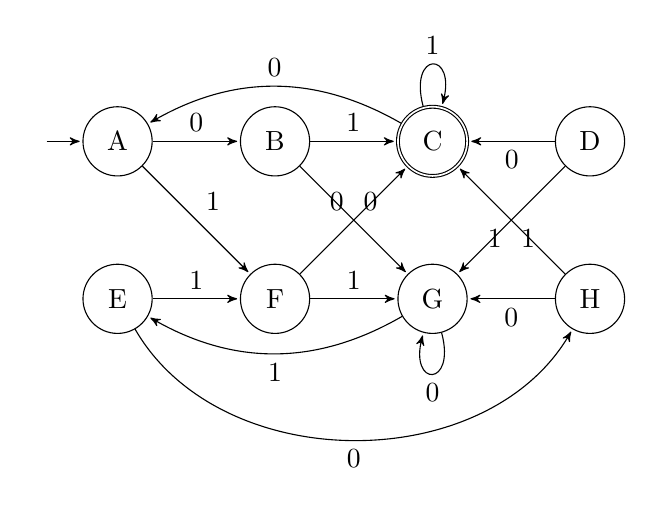
\begin{tikzpicture}[>=stealth',shorten >=1pt,auto,node distance=2cm]
                        % \useasboundingbox (-1,-2.50) rectangle (4,1);
                        % \scope[transform canvas={scale=1}]
                        \node[initial,state] (q0)      {A};
                        \node[state] (q1)  [right of=q0]     {B};
                        \node[state,accepting] (q2) [right of=q1]     {C};
                        \node[state] (q3) [right of=q2]     {D};
                        \node[state] (d0)  [below of=q0]    {E};
                        \node[state] (d1)  [right of=d0]     {F};
                        \node[state] (d2) [right of=d1]     {G};
                        \node[state] (d3) [right of=d2]     {H};
                        \path[->]
                            (q0)  edge  node {0} (q1)
                            (q0)  edge  node {1} (d1)
                            (q1)  edge  node {0} (d2)
                            (q1)  edge  node {1} (q2)
                            (q2)  edge[bend right]  node[swap] {0} (q0)
                            (q2)  edge[loop above]  node {1} (q2)
                            (q3)  edge  node {0} (q2)
                            (q3)  edge  node {1} (d2)
                            (d0)  edge[bend right=60]  node[swap] {0} (d3)
                            (d0)  edge  node {1} (d1)
                            (d1)  edge  node {0} (q2)
                            (d1)  edge  node {1} (d2)
                            (d2)  edge[loop below]  node {0} (d2)
                            (d2)  edge[bend left]  node {1} (d0)
                            (d3)  edge  node {0} (d2)
                            (d3)  edge  node {1} (q2);
                        % \endscope
                    \end{tikzpicture}
                }
            \end{center} 

            \column{0.5\textwidth}

            \small

            C, G distinguishable, $\delta^*(C,\lambda)\in{ F}$, $\delta^*(G,\lambda)\notin{ F}$

            \smallskip
                
            A,G too: $\delta^*(A,01)=C$ accepting, $\delta^*(G,01)=E$ not accepting.
            
            \smallskip

            A,E equivalent (for $\lambda$, $1*$ obvious, $0$ goes to non-accepting, $01$ \& $00$ meet in the same state)

        \end{columns}

    \end{example}
            
\end{frame}


\begin{frame}{Recognizing state equivalence}

    Distinguish accepting from nonaccepting. Then go backwards.
    
    \begin{algorithm}[Finding distinguishable states in a DFA]    
        \begin{itemize}
            \item \alert{Basis:} If $p\in { F}$ is accepting and $q\notin{ F}$ is not, the pair  $ \{p,q\}$ is distinguishable.
            \item \alert{Induction:} Let $p,q\in Q$ and $a\in \Sigma$. If $r=\delta(p,a)$ and $s=\delta(q,a)$ are distinguishable, then so are $p$ and $q$. (Repeat until no newly distinguished pair.)
        \end{itemize}
    \end{algorithm}

\end{frame}


\begin{frame}{Example 1/4}

    \begin{columns}

        \column{0.5\textwidth}

        1. Accepting vs. non--accepting

        \bigskip
            
        \begin{tabular}{c c c c c c c c}\cline{2-2}
            B & \nx \\ \cline{2-3}
            C &\x &  \x  \\ \cline{2-4}
            D &\nx &  \nx &  \x \\ \cline{2-5}
            E & \nx &  \nx & \x &  \nx \\ \cline{2-6}
            F & \nx & \nx &  \x &\nx &\nx \\ \cline{2-7}
            G & \nx & \nx &  \x &\nx &\nx &\nx\\ \cline{2-8}
            H & \nx & \nx & \x &  \nx &\nx &\nx &\nx\\ \cline{2-8}
            &A&B&C&D&E&F&G
        \end{tabular}            
        
        \column{0.5\textwidth}

        \begin{center}
            \scalebox{0.67}{
                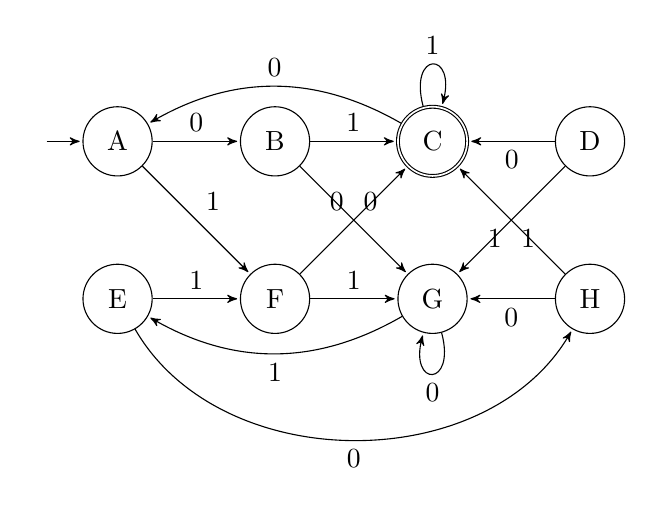
\begin{tikzpicture}[>=stealth',shorten >=1pt,auto,node distance=2cm]
                    % \useasboundingbox (-1,-2.50) rectangle (4,1);
                    % \scope[transform canvas={scale=1}]
                    \node[initial,state] (q0)      {A};
                    \node[state] (q1)  [right of=q0]     {B};
                    \node[state,accepting] (q2) [right of=q1]     {C};
                    \node[state] (q3) [right of=q2]     {D};
                    \node[state] (d0)  [below of=q0]    {E};
                    \node[state] (d1)  [right of=d0]     {F};
                    \node[state] (d2) [right of=d1]     {G};
                    \node[state] (d3) [right of=d2]     {H};
                    \path[->]
                        (q0)  edge  node {0} (q1)
                        (q0)  edge  node {1} (d1)
                        (q1)  edge  node {0} (d2)
                        (q1)  edge  node {1} (q2)
                        (q2)  edge[bend right]  node[swap] {0} (q0)
                        (q2)  edge[loop above]  node {1} (q2)
                        (q3)  edge  node {0} (q2)
                        (q3)  edge  node {1} (d2)
                        (d0)  edge[bend right=60]  node[swap] {0} (d3)
                        (d0)  edge  node {1} (d1)
                        (d1)  edge  node {0} (q2)
                        (d1)  edge  node {1} (d2)
                        (d2)  edge[loop below]  node {0} (d2)
                        (d2)  edge[bend left]  node {1} (d0)
                        (d3)  edge  node {0} (d2)
                        (d3)  edge  node {1} (q2);
                    % \endscope
                \end{tikzpicture}
            }
        \end{center}
                
    \end{columns}

\end{frame}


\begin{frame}{Example 2/4}

    \begin{columns}

        \column{0.5\textwidth}

        2. $\delta(q,1)\in{\mathcal F}$ for $q\in\{B,C,H\}$

        \bigskip
        
        \begin{tabular}{c c c c c c c c}\cline{2-2}
            B & \x \\ \cline{2-3}
            C &\x &  \x  \\ \cline{2-4}
            D &\nx &  \x &  \x \\ \cline{2-5}
            E & \nx &  \x & \x &  \nx \\ \cline{2-6}
            F & \nx & \x &  \x &\nx &\nx \\ \cline{2-7}
            G & \nx & \x &  \x &\nx &\nx &\nx\\ \cline{2-8}
            H & \x & \nx & \x &  \x &\x &\x &\x\\ \cline{2-8}
            &A&B&C&D&E&F&G
        \end{tabular}

        \column{0.5\textwidth}

        \begin{center}
            \scalebox{0.67}{
                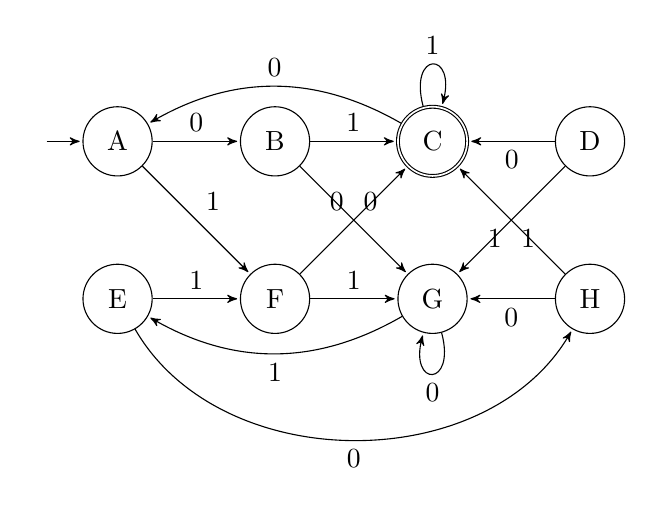
\begin{tikzpicture}[>=stealth',shorten >=1pt,auto,node distance=2cm]
                    % \useasboundingbox (-1,-2.50) rectangle (4,1);
                    % \scope[transform canvas={scale=1}]
                    \node[initial,state] (q0)      {A};
                    \node[state] (q1)  [right of=q0]     {B};
                    \node[state,accepting] (q2) [right of=q1]     {C};
                    \node[state] (q3) [right of=q2]     {D};
                    \node[state] (d0)  [below of=q0]    {E};
                    \node[state] (d1)  [right of=d0]     {F};
                    \node[state] (d2) [right of=d1]     {G};
                    \node[state] (d3) [right of=d2]     {H};
                    \path[->]
                        (q0)  edge  node {0} (q1)
                        (q0)  edge  node {1} (d1)
                        (q1)  edge  node {0} (d2)
                        (q1)  edge  node {1} (q2)
                        (q2)  edge[bend right]  node[swap] {0} (q0)
                        (q2)  edge[loop above]  node {1} (q2)
                        (q3)  edge  node {0} (q2)
                        (q3)  edge  node {1} (d2)
                        (d0)  edge[bend right=60]  node[swap] {0} (d3)
                        (d0)  edge  node {1} (d1)
                        (d1)  edge  node {0} (q2)
                        (d1)  edge  node {1} (d2)
                        (d2)  edge[loop below]  node {0} (d2)
                        (d2)  edge[bend left]  node {1} (d0)
                        (d3)  edge  node {0} (d2)
                        (d3)  edge  node {1} (q2);
                    % \endscope
                \end{tikzpicture}
            }
        \end{center}
                
    \end{columns}

\end{frame}


\begin{frame}{Example 3/4}

    \begin{columns}

        \column{0.5\textwidth}

        3. $\delta(q,0)\in{\mathcal F}$ for $q\in\{D,F\}$

        \bigskip
        
        \begin{tabular}{c c c c c c c c}\cline{2-2}
            B & \x \\ \cline{2-3}
            C &\x &  \x  \\ \cline{2-4}
            D &\x &  \x &  \x \\ \cline{2-5}
            E & \nx &  \x & \x &  \x \\ \cline{2-6}
            F & \x & \x &  \x &\nx &\x \\ \cline{2-7}
            G & \nx & \x &  \x &\x &\nx &\x\\ \cline{2-8}
            H & \x & \nx & \x &  \x &\x &\x &\x\\ \cline{2-8}
            &A&B&C&D&E&F&G
        \end{tabular}

        \column{0.5\textwidth}

        \begin{center}
            \scalebox{0.67}{
                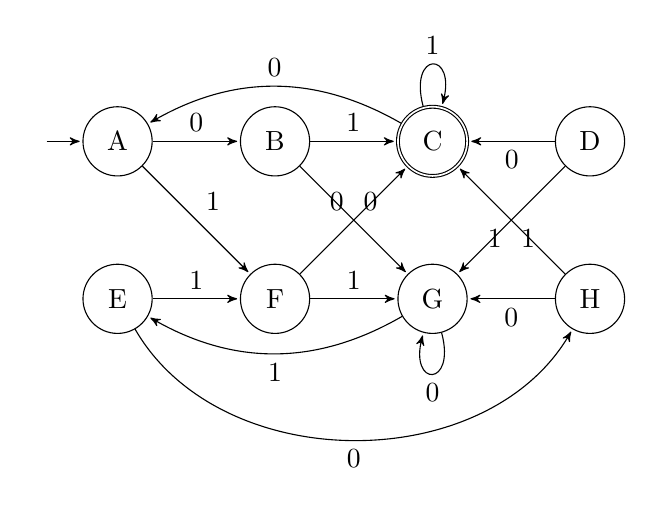
\begin{tikzpicture}[>=stealth',shorten >=1pt,auto,node distance=2cm]
                    % \useasboundingbox (-1,-2.50) rectangle (4,1);
                    % \scope[transform canvas={scale=1}]
                    \node[initial,state] (q0)      {A};
                    \node[state] (q1)  [right of=q0]     {B};
                    \node[state,accepting] (q2) [right of=q1]     {C};
                    \node[state] (q3) [right of=q2]     {D};
                    \node[state] (d0)  [below of=q0]    {E};
                    \node[state] (d1)  [right of=d0]     {F};
                    \node[state] (d2) [right of=d1]     {G};
                    \node[state] (d3) [right of=d2]     {H};
                    \path[->]
                        (q0)  edge  node {0} (q1)
                        (q0)  edge  node {1} (d1)
                        (q1)  edge  node {0} (d2)
                        (q1)  edge  node {1} (q2)
                        (q2)  edge[bend right]  node[swap] {0} (q0)
                        (q2)  edge[loop above]  node {1} (q2)
                        (q3)  edge  node {0} (q2)
                        (q3)  edge  node {1} (d2)
                        (d0)  edge[bend right=60]  node[swap] {0} (d3)
                        (d0)  edge  node {1} (d1)
                        (d1)  edge  node {0} (q2)
                        (d1)  edge  node {1} (d2)
                        (d2)  edge[loop below]  node {0} (d2)
                        (d2)  edge[bend left]  node {1} (d0)
                        (d3)  edge  node {0} (d2)
                        (d3)  edge  node {1} (q2);
                    % \endscope
                \end{tikzpicture}
            }
        \end{center}
                
    \end{columns}

\end{frame}


\begin{frame}{Example 4/4}

    \begin{columns}

        \column{0.5\textwidth}

        4. $B$ and $G$ are distinguishable, $\delta(A,0)=B$, $\delta(G,0)=G$, therefore $A,G$ are distinguishable.
            Similarly, $\delta(*,0)$ for $E,G$ goes to distinguishable states $H,G$. 

        \bigskip
                
        \begin{tabular}{c c c c c c c c}\cline{2-2}
            B & \x \\ \cline{2-3}
            C &\x &  \x  \\ \cline{2-4}
            D &\x &  \x &  \x \\ \cline{2-5}
            E & \nx &  \x & \x &  \x \\ \cline{2-6}
            F & \x & \x &  \x &\nx &\x \\ \cline{2-7}
            G & \x & \x &  \x &\x &\x &\x\\ \cline{2-8}
            H & \x & \nx & \x &  \x &\x &\x &\x\\ \cline{2-8}
            &A&B&C&D&E&F&G
        \end{tabular}

        \column{0.5\textwidth}

        \begin{center}
            \scalebox{0.67}{
                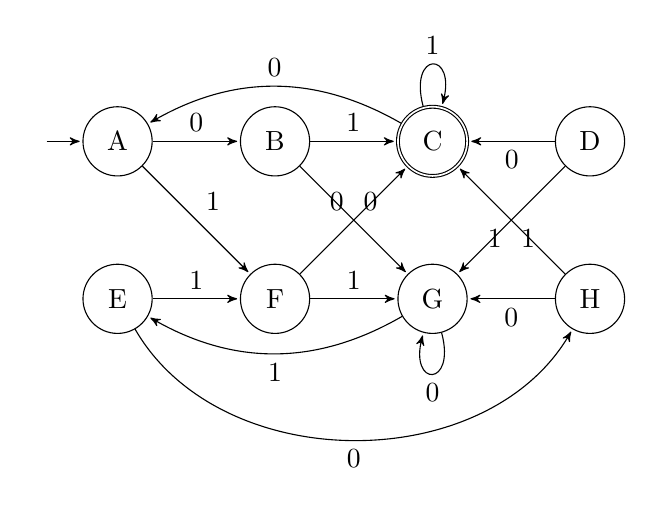
\begin{tikzpicture}[>=stealth',shorten >=1pt,auto,node distance=2cm]
                    % \useasboundingbox (-1,-2.50) rectangle (4,1);
                    % \scope[transform canvas={scale=1}]
                    \node[initial,state] (q0)      {A};
                    \node[state] (q1)  [right of=q0]     {B};
                    \node[state,accepting] (q2) [right of=q1]     {C};
                    \node[state] (q3) [right of=q2]     {D};
                    \node[state] (d0)  [below of=q0]    {E};
                    \node[state] (d1)  [right of=d0]     {F};
                    \node[state] (d2) [right of=d1]     {G};
                    \node[state] (d3) [right of=d2]     {H};
                    \path[->]
                        (q0)  edge  node {0} (q1)
                        (q0)  edge  node {1} (d1)
                        (q1)  edge  node {0} (d2)
                        (q1)  edge  node {1} (q2)
                        (q2)  edge[bend right]  node[swap] {0} (q0)
                        (q2)  edge[loop above]  node {1} (q2)
                        (q3)  edge  node {0} (q2)
                        (q3)  edge  node {1} (d2)
                        (d0)  edge[bend right=60]  node[swap] {0} (d3)
                        (d0)  edge  node {1} (d1)
                        (d1)  edge  node {0} (q2)
                        (d1)  edge  node {1} (d2)
                        (d2)  edge[loop below]  node {0} (d2)
                        (d2)  edge[bend left]  node {1} (d0)
                        (d3)  edge  node {0} (d2)
                        (d3)  edge  node {1} (q2);
                    % \endscope
                \end{tikzpicture}
            }

            \bigskip

            Equivalent pairs: 
                
            \bigskip

            \alert{$(A,E)$, $(B,H)$, $(D,F)$}

        \end{center}
            
    \end{columns}

\end{frame}


\begin{frame}{Correctness}

    \begin{theorem}
        A pair of states is not distinguished by the algorithm, if and only if the states are equivalent.
    \end{theorem}
    \begin{proof}
        \alert{\Large$\Leftarrow$} Clearly, only distinguishable pairs are distinguished.\\ 
        \alert{\Large$\Rightarrow$} Induction on the length of a shortest distinguishing word. If $p,q$ are distinguished by $w=\epsilon$, then the algorithm distinguishes them. Now let $w=a_1\ldots a_k$. By induction, $r=\delta(p,a_1)$ and $s=\delta(q,a_1)$ are distinguished by the algorithm. But then the algorithm distinguishes $p,q$ in the next round (following $a_1$-transitions backwards).
    \end{proof}        
    
\end{frame}


\begin{frame}{Complexity}

    
    The time complexity is polynomial in the number of states $n$.
    \begin{itemize}
        \item In one iteration, we consider all pairs, that is $O(n^2)$.
        \item In each iteration we add a cross, that means no more than  $O(n^2)$ iterations.
        \item Together, $O(n^4)$.
    \end{itemize}
    The algorithm may be sped up to $O(n^2)$ by memorizing states that depend on the pair $\{r,s\}$ and following the list backwards.

        
    \begin{exercise}
        \begin{itemize}
            \item Describe the $O(n^2)$ algorithm hinted above.    
            \item The algorithm can also compute, for each distinguishable pair, the shortest word distinguishing that pair.
        \end{itemize}
    \end{exercise}
    
\end{frame}


\begin{frame}{Application: testing equality of regular languages}

    \begin{itemize}
        \item regular languages $L,M$ are given by some representations
        \item from those construct DFA $A_L,A_M$ recognizing $L,M$
        \item we can assume $Q_L\cap Q_L=\emptyset$ (otherwise rename the states)
        \item run the following algorithm:
    \end{itemize}
    
    \begin{algorithm}[Testing equivalence of automata]
        \begin{itemize}
            \item Construct a DFA \alert{$B=(Q_L\cup Q_M, \Sigma, \delta_L\cup \delta_M,q_L, F_L\cup F_M)$} as a union of states and transitions; select one (any) initial state.
            \item Test if ${q_{0}}_L$ and ${q_{0}}_M$ are equivalent.
            (The automata are equivalent iff their initial states are equivalent in $B$.)                
        \end{itemize}
    \end{algorithm}
        
    \textbf{NB:} Renaming states gives an isomorphic (hence equivalent) automaton. So we can always assume disjoint states. Alternatively, we can use disjoint union: $Q_B=Q_L\dot\sqcup Q_M=Q_L\times\{0\}\cup Q_M\times\{1\}$.
    
\end{frame}


\begin{frame}{Example}

    \begin{example}
        Two different DFAs recognizing $L=\{\lambda\}\cup \{w0\mid w\in\{0,1\}^*\}$.
    \end{example}

    \begin{columns}

        \column{0.5\textwidth}

        \begin{center}
            \scalebox{1}{
                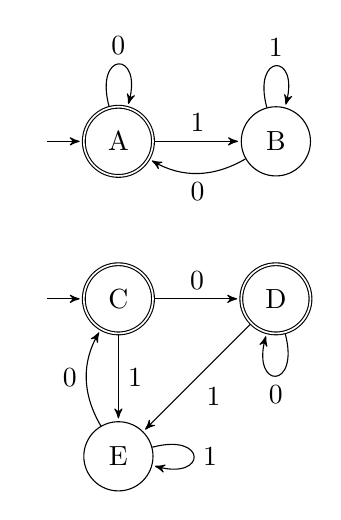
\begin{tikzpicture}[]                
                    \node[initial,state,accepting] (q0)      {A};
                    \node[state] (q1)  [right of=q0]     {B};
                    \node[initial,state,accepting] (c)  [below of=q0]    {C};
                    \node[state,accepting] (d)  [right of=c]     {D};
                    \node[state] (e) [below of=c]    {E};
                    \path[->]
                        (q0)  edge[loop above]  node {0} (q0)
                        (q0)  edge  node {1} (q1)
                        (q1)  edge[loop above]  node {1} (q0)
                        (q1)  edge[bend left]  node {0} (q0)
                        (c)  edge  node {0} (d)
                        (c)  edge  node {1} (e)
                        (d)  edge[loop below]  node {0} (d)
                        (d)  edge  node {1} (e)
                        (e)  edge[loop right] node {1} (e)
                        (e)  edge[bend left] node {0} (c)
                    ;
                \end{tikzpicture}
            }
        \end{center}

        \column{0.5\textwidth}

        \begin{tabular}{c c c c c c}\cline{2-2}
            B & \x \\ \cline{2-3}
            C &\nx &  \x  \\ \cline{2-4}
            D &\nx &  \x &  \nx \\ \cline{2-5}
            E & \x &  \nx & \x &  \x \\ \cline{2-6}
            &A&B&C&D
        \end{tabular}       
        
    \end{columns}

\end{frame}


\begin{frame}{Reduced automaton}
    
    \begin{definition}[Reduced DFA]
        A DFA $A$ is \alert{reduced} iff all states are reachable, no two distinct states are equivalent, and there is no `fail' state from which no accepting state would be reachable. 
        
        It is a \alert{reduct of} a DFA $B$ iff it is reduced and equivalent to $B$.
    \end{definition}

    \begin{theorem}[DFA minimization]
        \begin{enumerate}[(i)]
            \item Any two equivalent reduced automata are isomorphic.
            \item Any DFA accepting at least one word has a reduct, unique up to automata isomorphism.            
        \end{enumerate}        
    \end{theorem}
    \begin{proof}
        \alert{(i)} Any $q\in Q_1$ is reachable. Find a word $w$ s.t. $q=\delta_1^*(q_{0_1},w)$. Define $h(q)=\delta_2^*(q_{0_2},w)$. Check that $h$ is an isomorphism. \\ \alert{(ii)} The construction described on the next slide works.        
    \end{proof}

\end{frame}


\begin{frame}{Algorithm: constructing the reduct}
    
    \textbf{input:} a DFA $B$\\
    \textbf{output:} a DFA $A$ which is the reduct of $B$

    \begin{enumerate}
        \item eliminate from $B$ all unreachable states
        \item find the indistinguishability partition on the remaining states
        \item construct the reduct $B$:
    \end{enumerate}
    \begin{itemize}
        \item $Q_B$ are the equivalence classes
        \item $q_{0_B}$ is the class containing the initial state of $A$
        \item final states $F_B$ are the classes containing some state from $F_A$
        \item the \alert{transition function}: for any $a\in\Sigma$ and $S\in Q_B$ choose arbitrary $q\in S$ and define \alert{$\delta_B(S,a)=[\delta_A(q,a)]$}, i.e., the class containing  $\delta_A(q,a)\in Q_A$; note that this class is the same for any choice of $q\in S$ since they are all equivalent
        \item if there's a `fail' state from which no final states can be reached [and if we allow partial transition functions], remove it
    \end{itemize}

\end{frame}


\begin{frame}{Example}

    \begin{multicols}{2}
        
        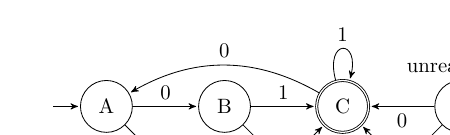
\begin{tikzpicture}[>=stealth',shorten >=1pt,auto,node distance=2cm]
            \useasboundingbox (-1,0) rectangle (4,1);
            \scope[transform canvas={scale=0.75}]
                \node[initial,state] (q0)      {A};
                \node[state] (q1)  [right of=q0]     {B};
                \node[state,accepting] (q2) [right of=q1]     {C};
                \node[state,label=above:{unreachable}] (q3) [right of=q2]     {D};
                \node[state] (d0)  [below of=q0]    {E};
                \node[state] (d1)  [right of=d0]     {F};
                \node[state] (d2) [right of=d1]     {G};
                \node[state] (d3) [right of=d2]     {H};
                \path[->]
                    (q0)  edge  node {0} (q1)
                    (q0)  edge  node {1} (d1)
                    (q1)  edge  node {0} (d2)
                    (q1)  edge  node {1} (q2)
                    (q2)  edge[bend right]  node[swap] {0} (q0)
                    (q2)  edge[loop above]  node {1} (q2)
                    (q3)  edge  node {0} (q2)
                    (q3)  edge  node {1} (d2)
                    (d0)  edge[bend right]  node[swap] {0} (d3)
                    (d0)  edge  node {1} (d1)
                    (d1)  edge  node {0} (q2)
                    (d1)  edge  node {1} (d2)
                    (d2)  edge[loop below]  node {0} (d2)
                    (d2)  edge[bend left]  node {1} (d0)
                    (d3)  edge  node {0} (d2)
                    (d3)  edge  node {1} (q2)
                ;
            \endscope
        \end{tikzpicture} 
       
        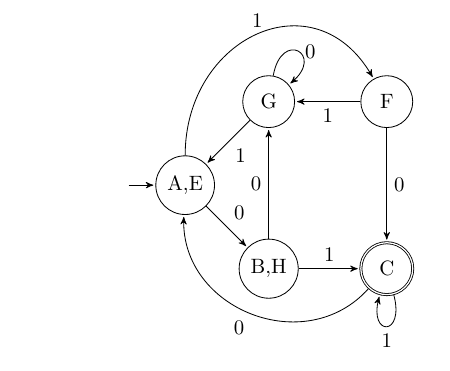
\begin{tikzpicture}[>=stealth',shorten >=1pt,auto,node distance=2cm]
            \useasboundingbox (-2,-2) rectangle (3,2);
            \scope[transform canvas={scale=0.75}]
                \node[initial,state] (ae)      {A,E};
                \node[state] (g)  [above right of=ae]     {G};
                \node[state] (bh)  [below right of=ae]    {B,H};
                \node[state] (df)  [right of=g]     {F};
                \node[state, accepting] (c)   [right of=bh]   {C};
                \path[->]
                    (g)  edge[in=40,out=80,distance=0.8cm,right]  node {0} (g)
                    (ae)  edge  node {0} (bh)
                    (ae)  edge[in=120,out=90,above,distance=2cm]  node {1} (df)
                    (c)  edge[loop below]  node {1} (c)
                    (g)  edge  node {1} (ae)
                    (df)  edge  node {1} (g)
                    (df)  edge  node {0} (c)
                    (c)  edge[bend left=70,distance=1.6cm]  node {0} (ae)
                    (bh)  edge  node {1} (c)
                    (bh)  edge  node {0} (g)
                ;
            \endscope
        \end{tikzpicture}
        \end{multicols}       

    \begin{multicols}{2}

        {\scriptsize %footnotesize %small
            \begin{tabular}{c c c c c c c}\cline{2-2}
            B & \x \\ \cline{2-3}
            C &\x &  \x  \\ \cline{2-4}
            E & \nx &  \x & \x  \\ \cline{2-5}
            F & \x & \x &  \x  &\x \\ \cline{2-6}
            G & \x & \x &  \x  &\x &\x\\ \cline{2-7}
            H & \x & \nx & \x  &\x &\x &\x\\ \cline{2-7}
            &A&B&C&E&F&G
            \end{tabular}
        }

        Equivalence classes:
        $$
        \{A,E\},\{B,H\},\{C\},\{F\},\{G\}
        $$
    \end{multicols}

\end{frame}


\begin{frame}{Summary of Lecture 2}

    \begin{itemize}
        \item \alert{Mihyll–Nerode theorem} (DFAs $\leftrightarrow$ right congruences of $\Sigma^*$ of finite index where $L$ is a union of classes)
        \item Equivalent automata (recognize the same language), automata homomorphism (implies automata equivalence).
        \item Finding reachable states: BFS on the state diagram
        \item Finding equivalent (indistinguishable) states: a table-filling algorithm
        \item Testing equivalence of DFAs, equality of regular languages
        \item Reduced (minimum–state) DFA, an algorithm to reduce a given DFA (using the equivalent states algorithm)
    \end{itemize}

\end{frame}



\end{document}
